\chapter{Installation}\label{cha:installation}

\section{Compatibility}

\subsection{Devices for running XCSoar}

XCSoar runs on the following platforms:

\begin{itemize}
\item mobile phones and tablets with Android 1.6 or newer \\
  Example: Dell Streak, Samsung Galaxy S II, HTC Desire HD,
  Motorola Xoom
\item PDAs with Pocket PC 2000, 2002, 2003 \\
  Example: iPaq 3800, iPaq 3900
\item PDAs with Windows Mobile \\
  Example: iPaq hx4700, Dell Axim x51v
\item PNAs with Windows CE 3.0 or newer \\
  Example: HP314, Mio400
\item Triadis Altair
\item LX MiniMap
\item Windows 2000 or newer
\item Linux
\end{itemize}

\subsection{Sensors, Loggers, Varios}

XCSoar is compatible with any GPS emitting NMEA data.  Most modern
Android devices have a built-in GPS, but sometimes it is favorable to
connect to an external device:

\begin{itemize}
\item an airspeed indicator allows quick and exact wind estimates
\item a vario improves the thermal assistant
\item a task can be declared to an IGC logger, and after landing, the
  flight log can be downloaded
\item some varios allow synchronising the MacCready setting with
  XCSoar
\end{itemize}

\begin{figure}
\begin{tabular}{l|cccc}

Product & Airspeed & Vario & Declaration & Download \\

\hline

Borgelt B50 & $\surd$ \\

CAI 302 & $\surd$ & $\surd$ & $\surd$ & $\surd$ \\

CAI GPS Nav \\

Condor & $\surd$ \\

Digifly Leonardo & $\surd$ & $\surd$ \\

EW Logger &&& $\surd$ \\

EW microRecorder &&& $\surd$ \\

Flymaster F1 && $\surd$ \\

Flytec 5030 & $\surd$ & $\surd$ \\

ILEC SN10 & & $\surd$ \\

IMI ERIXX &&& $\surd$ & $\surd$ \\

LX20, Colibri &&& $\surd$ & $\surd$ \\

LX 5000, 7000 & $\surd$ & $\surd$ & $\surd$ \\

PosiGraph &&& $\surd$ \\

Triadis Altair &&& $\surd$ \\

Triadis Vega & $\surd$ & $\surd$ \\

Volkslogger &&& $\surd$ \\

Westerboer VW1150 & $\surd$ & $\surd$ \\

Zander / SDI & $\surd$ & $\surd$ \\

\end{tabular}
\caption{Supported external devices and some of their features}
\end{figure}

While most Windows CE based devices have a serial port, such legacy
hardware is not present in modern Android devices.  Those can either
use Bluetooth or the Android IOIO board.  To use Bluetooth, you need
to connect the external device to a Bluetooth-to-Serial adapter, such
as the K6-Bt or the Glidertools VFBT-1.

\section{Downloading XCSoar}
The software is available as a free download from the XCSoar website
~\xcsoarwebsite. Follow the links to the download section.

\subsection*{Pocket PC versions}
Download the relevant package for your Pocket PC operating system
version and save it to disk:
\begin{description}
\item[Pocket PC 2000] For Pocket PC 2002 and older
\item[Windows Mobile 2003] For Windows Mobile 2003 (or Pocket PC 2003)
\item[Windows Mobile 5] For Windows Mobile 5 and 6
\end{description}

\subsection*{Data files location}
To be able to use XCSoar's advanced features, additional data files, such as
terrain, topography, special use airspace, waypoints etc.\ are needed. The files
that can be used with XCSoar are described in Chapter~\ref{cha:data-files}.

All data files should be copied into the directory
\texttt{XCSoarData}.  This directory must be in a specific place
so that XCSoar knows where to look for data files:

\begin{description}
\item[Windows PC]
\texttt{XCSoarData} must be located in your personal folder (``\texttt{My
Documents}'')
\item[Windows Mobile PDA/PNA]
\begin{itemize}
\item If you start XCSoar from a SD card, it is always in the root of
  that SD card (e.g. ``\texttt{SD Card/XCSoarData}'')
\item If \texttt{XCSoarData} already exists on any SD card inserted
  at XCSoar start\-up, this one is used.
\item If none of the above applies, then it is in your personal folder
  (``\texttt{My Documents/}'')
\end{itemize}
\item[Unix PC]
\verb|~/.xcsoar/XCSoarData|.
\item[Android Devices]
\texttt{XCSoarData} is located on the SD card (e.g.
``\texttt{/sdcard/XCSoarData}'').
\item[Altair]
If XCSoarData exists on an USB drive, that one is used, otherwise the
internal storage is used.
\end{description}

For embedded devices it is recommended to create \texttt{XCSoarData} on a SD
card, because you can easily update the data files using your PC.


XCSoar will generate a number of additional files at run time.  These
will be placed in the  \texttt{XCSoarData} directory (Windows PC and 
Windows Mobile devices), or the \texttt{.xcsoar} directory (Unix/Linux
PC).  At first run, XCSoar will create the files 
\texttt{Default.tsk} (Default Task),  \texttt{xcsoar-registry.prf} 
(configuration settings), \newline
\texttt{xcsoar-startup.log} (log of the startup progress), 
plus three directories: \texttt{cache},
\texttt{config} and \texttt{logs}.  Additional files may be
created/modified while XCSoar is running, such as task files
(\texttt{*.tsk}) and flight logs.




\section{Installation}
\subsection*{Installation of Pocket PC version from Windows PC}

Prior to performing any installation, it is a good idea to backup your
organiser for extra safety.

The following sequence describes how to install XCSoar from Windows:
\begin{enumerate}
\item Place your PocketPC in its cradle and make sure
 you have MS ActiveSync running.
\begin{center}
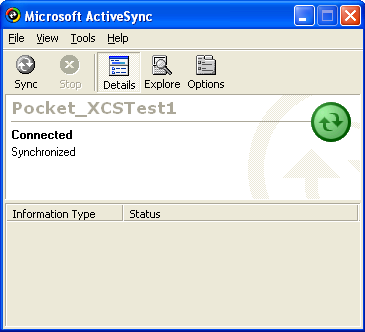
\includegraphics[angle=0,width=\linewidth,keepaspectratio='true']{figures/XCS_ActiveSync.png}
\end{center}

\item Run the program \verb|Install-XCSoar-XXX-YYY.exe| 
  (where XXX and YYY refer to the version number and operating system
  version respectively).

\begin{center}
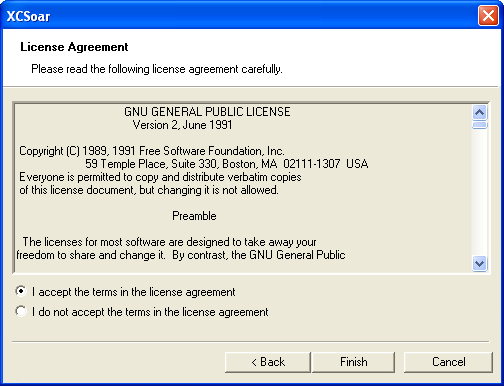
\includegraphics[angle=0,width=\linewidth,keepaspectratio='true']{figures/XCS_License.png}
\end{center}

\item Read and accept the license
\item Follow the prompts in the installation program and also follow the prompts on the organiser.

\begin{center}
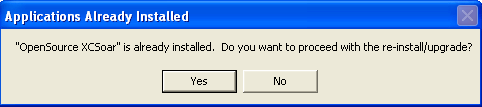
\includegraphics[angle=0,width=\linewidth,keepaspectratio='true']{figures/XCS_Windows.png}
\end{center}

\item XCSoar is now installed.
\item Perform a reset of your device.  See the operating instructions for your
  organiser about how to do this.
\item After the reset, the XCSoar `FLY' and `SIM' launcher icons will
 be visible on the Today screen.

\begin{center}
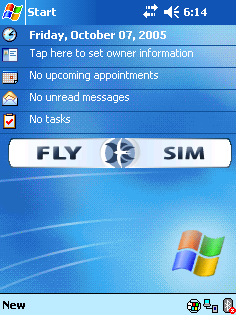
\includegraphics[angle=0,width=0.6\linewidth,keepaspectratio='true']{figures/XCS_Today.png}
\end{center}

\end{enumerate}

It is a good idea to assign one of your PocketPC hardware buttons to
run XCSoar. See your PocketPC manual for details of how to do this.

Owners of Compaq Aero PocketPCs may find it useful to enable `Game
Keys'.

\subsection*{Installation of Pocket PC version from a Pocket PC CAB file}

You can download the CAB file appropriate for your organiser and
install it onto a nonvolatile storage card like a Compact Flash or
Secure Digital card. Place it in your organiser. Use the File Manager
on your organiser to find the CAB and click on it to execute
it. Follow the on-screen instructions, the CAB file will be deleted
after installation.

Alternatively you can download the CAB file from Sourceforge through
your Internet Explorer on your organiser and install it that way.

\tip It is generally a good idea to keep the CAB file on the storage card
so that if the organiser's power fails and the memory is lost, XCSoar
can be reinstalled.

\subsection*{Installation of PC version}

The file \verb|XCSoarPC.zip| needs to be unzipped using a utility
program such as WinZip.

Development of a proper windows installer for the PC version is in
progress.  For now, any additional data files used by the PC version
must be placed in the \verb|My Documents\XCSoarData| directory.


\subsection*{Installation on Unix/Linux}

The file downloaded is \verb|xcsoar_XXX.deb|, where \verb|XXX| includes
the version number and platform, e.g. \verb|xcsoar_6.0.4_i386.deb|.
The is a Debian package and can be installed using 
\begin{center}
\verb|sudo dpkg -i xcsoar_XXX.deb|.
\end{center}
Use \verb|dpkg-query -L xcsoar| to see where the executable and 
other files are installed,
Additional data files must be placed in the directory
\verb|~/.xcsoar/XCSoarData/|.
If \verb|~/.xcsoar| does not exist, it will be created the first time
that \verb|xcsoar| is run.


\subsection*{Installation on Android}

Obtain XCSoar from Google's Android market, or install the \verb|apk|
file manually.  Copy the data files on the SD card in the directory
\verb|XCSoarData|.


\section{Running XCSoar}
%\subsection*{Fly and simulator modes}

Two modes are available inside the XCSoar application: 
\begin{description}
\item[FLY] This mode is used when actually flying.  The simulator is 
  disabled and serial communications are active. 
\item[SIM] This starts XCSoar in simulator mode, no serial communications
  are attempted.
\end{description}

\subsection*{XCSoar Pocket PC version}
The program can be run in either of two modes by pressing the `FLY' or
`SIM' launcher on the Today screen. If the application is started directly from
the explorer a dialog is asking you which mode you want to start.

\tip It is recommended that on Pocket PC devices, no other programs
 are running while XCSoar is used in flights.  This gives the best
 possible performance and responsiveness of the program.

\subsection*{Altair version}
XCSoar starts up automatically when Altair is powered on.
The PWR/ESC button (top left) has multiple functions:
\begin{description}
\item[Powering on]  Press and hold the PWR/ESC button for one second.
  The LED in the button will light up, and XCSoar will start after
  Altair has booted.
\item[Powering off]  Press and hold the PWR/ESC button for 3 seconds.
  Altair will switch off.
\item[Escape] Pressing the PWR/ESC button quickly acts as an
Escape key, typically used to close dialog pages or as a cancel function.
\end{description}

The Altair version of XCSoar does not include a simulator mode.

\subsection*{XCSoar PC version}
The program can be run by opening the explorer window, finding the directory
that has the XCSoar.exe executable, and double clicking on that program file.

The program command line options allows the screen orientation of
the display to be defined:
\begin{description}
\item[-portrait] The screen is 480 pixels wide, 640 pixels high.
\item[-square] The screen is 480 pixels wide, 480 pixels high.
\item[-landscape] The screen is 640 pixels wide, 480 pixels high. This is the
usual setting. If you don't specify this parameter the landscape version will be
loaded automatically.
\item[-small] Draws the screen at half size.  This is useful for using XCSoar in
 conjunction with flight simulators e.g.\ Condor.
\end{description}
To change the screen orientation, it is convenient to create a shortcut to the
program, then right click on the shortcut icon and click on ``Shortcut''. 
In the field ``Target'' add one of the desired options listed above.

\subsection*{XCSoar Unix/Linux PC version}
Run \verb|xcsoar| from a command line, or create a shortcut on the
desktop.  The location of the executable file may be found using
\verb|which xcsoar|.  Only landscape mode is  supported for now.

\subsection*{Loading data files}
The first time that XCSoar is run, it does not automatically load the 
data files that you placed in the \verb|XCSoarData| directory.  
To tell XCSoar which files to load, double click/tap the map (the large,
blank white part with the glider symbol in the center),
choose the menu \bmenu{Config} (click/tap it twice), then select
\bmenu{System Setup}.  The System Setup screen should be displayed:
\begin{center}
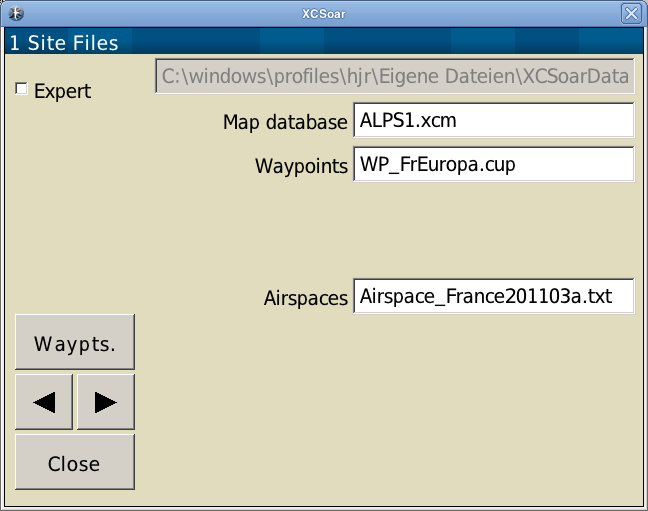
\includegraphics[angle=0,width=0.8\linewidth,keepaspectratio='true']{figures/config-basic.png}
\end{center}
The first page allows you to choose the map, 
waypoint and airspace files, by clicking/tapping on the text boxes.
Many other features of XCSoar may be configured with
\bmenu{System Setup}. These are described in detail in Chapter
\ref{cha:configuration}.
Once completed, XCSoar must be restarted; from now on, the data files
will be loaded automatically at run time.

\subsection*{Start-up and user profiles}
When XCSoar starts up, it will check for existing profiles. If multiple
profiles are detected it will displays a small window asking you which profile
to load. To proceed, choose the desired profile and press Enter. If no
profile is chosen the settings from the last session are loaded again. Profiles
can be useful for example in the following cases:
\begin{itemize}
\item Different pilots
\item Competition versus casual flying
\item Flying in different locations
\end{itemize}


\subsection*{SIM mode}
The simulator contains a simple interface allowing the user to fly
the glider about.  On the map screen, clicking/touching the glider symbol
(with touchscreen or mouse) and dragging 
causes the glider to move in the direction of the drag, the
speed being proportional to the length of the drag.  

In the PC version and for embedded devices with buttons, the aircraft
speed, height and direction may be changed using the \InfoBox es.
These features are not available for touchscreen devices.
The aircraft altitude can be adjusted by selecting the GPS altitude
{\InfoBox} (marked \infobox{H GPS}), and pressing the up or down key.
The airspeed  can be adjusted by selecting the ground speed
{\InfoBox} (marked \infobox{V Gnd}), and pressing the up or down key.
The glider's track  can be adjusted by selecting the track
{\InfoBox} (marked \infobox{Track}), and pressing the up or down key.
With either of the \InfoBox es \infobox{H GPS} or \infobox{V Gnd})
selected, the glider's direction may be changed using the left/right keys.

Other controls, buttons and menus work the same as in FLY mode.


\subsection*{Splash screen}
When XCSoar starts up, shuts down, or loads large files, such as airspace,
waypoints, terrain, etc., a progress screen is presented while the data is being
loaded. This screen has a progress bar which indicates the data loading
activity, and a short line of text describing the action that is being performed.

This screen also displays the software version information.

\subsection*{Exiting the program}
For PDA and PC versions, XCSoar is shut down from the menu. The menu can be
opened by double-clicking on the map or the \InfoBox es.
\begin{quote}
\bmenu{QUIT}
\end{quote}

For PC versions, XCSoar can also be shut down by clicking the close icon
on the XCSoar window.

For Altair, XCSoar is shut down by holding the PWR button for two seconds or
more.

